% !TeX program = pdflatex
\documentclass[11pt]{article}

\usepackage[margin=1in]{geometry}
\usepackage{lmodern}
\usepackage{microtype}
\usepackage{setspace}
\setstretch{1.08}
\usepackage{amsmath,amssymb,mathtools,bm,booktabs,tabularx,array,amsthm,longtable}
\usepackage{graphicx}
\usepackage{float}
\usepackage{tikz}
\usetikzlibrary{arrows.meta,positioning}
\usepackage{enumitem}
\usepackage[round,authoryear]{natbib}
\usepackage{hyperref}
\hypersetup{
  colorlinks=true,
  linkcolor=black,
  citecolor=black,
  urlcolor=black,
  pdftitle={Supplementary Material: Mean-Tilted Intervals: Short Tolerance Intervals},
  pdfauthor={Antonio De Leon, Raquel Prado, and Bruno Sanso}
}

\newcommand{\R}{\mathbb{R}}
\newcommand{\E}{\mathbb{E}}
\newcommand{\Normal}{\mathcal{N}}
\newcommand{\Exp}{\mathrm{Exp}}
\newcommand{\GIG}{\mathrm{GIG}}
\newcommand{\ind}{\mathbf{1}}
\newcommand{\diag}{\mathrm{diag}}
\newcommand{\vect}[1]{\bm{#1}}
\newcommand{\mat}[1]{\bm{#1}}
\newcommand{\RHS}{\mathrm{RHS}}
\newcommand{\TableStyle}{\footnotesize\setlength{\tabcolsep}{4pt}\renewcommand{\arraystretch}{1.08}}
\DeclareMathOperator{\argmin}{arg\,min}
\newtheorem{proposition}{Proposition}
\newtheorem{lemma}{Lemma}
\newtheorem{theorem}{Theorem}
\renewcommand{\theproposition}{S\arabic{proposition}}
\renewcommand{\thelemma}{S\arabic{lemma}}
\renewcommand{\thetheorem}{S\arabic{theorem}}
\newcounter{algorithm}
\renewcommand{\thealgorithm}{S\arabic{algorithm}}
\newenvironment{algorithmblock}[1]{%
  \refstepcounter{algorithm}\par\medskip
  \noindent\textbf{Algorithm \thealgorithm. #1}\par
  \begin{enumerate}[leftmargin=2.2em,itemsep=0.25em,parsep=0pt]%
}{%
  \end{enumerate}\par\medskip
}

\renewcommand{\theequation}{S\arabic{equation}}
\renewcommand{\thetable}{S\arabic{table}}
\renewcommand{\thefigure}{S\arabic{figure}}
\renewcommand{\thesection}{S\arabic{section}}
\renewcommand{\thesubsection}{S\arabic{section}.\arabic{subsection}}
\renewcommand{\thepage}{S\arabic{page}}

\title{Supplementary Material for \emph{Mean-Tilted Intervals:
Short Tolerance Intervals}}
\author{Antonio De Leon \and Raquel Prado \and Bruno Sans\'o}
\date{}

\begin{document}
\maketitle

\begin{abstract}
\noindent
This supplement gives the mathematical details and validation records for
\emph{Mean-Tilted Intervals: Short Tolerance Intervals}. It develops the
fixed-content interval class, the mean-preserving interval (MPI), and the
mean-tilted interval (MTI) family. It then records the finite-sample score
balance used to interpret fixed-target fits, the pseudo-asymmetric-Laplace
construction used by the MTI-ECM mode calculation, the direct
Dirichlet-process content-probability check, and the iid tolerance-validation
protocol. Endpoint regression, fixed-feature readouts, time-varying endpoint
models, and broader Gibbs computation are treated in a companion computation
paper.
\end{abstract}

\section*{Part I. Notation, Inferential Objects, and Guide to Supporting Results}

\section{Guide to the Supplement}
\label{sec:supp-guide}

The main article presents the statistical argument. This supplement gives the
recoverable derivations, fixed-target computational identities, and validation
records needed to support the tolerance claims. Throughout, MPI denotes the
zero-tilt retained-mean target and MTI denotes the fixed-content placement
family indexed by retained-mean tilt. TCSP denotes the scan-calibrated shortest
path tolerance action. The generalized posterior is always a loss-based update
for a fixed interval target; it is distinct from a response-distribution model
for \(F\).

\begin{table}[H]
\centering
\caption{\textbf{Notation used in the tolerance supplement.}}
\label{tab:supp-notation}
\TableStyle
\begin{tabularx}{\textwidth}{@{}l>{\raggedright\arraybackslash}X
  >{\raggedright\arraybackslash}X@{}}
\toprule
Symbol & Meaning & Use\\
\midrule
\(c\) & requested population content & fixed-content targets and tolerance actions\\
\(u\) & lower probability index for a content-\(c\) population window & interval paths\\
\(m,h\) & midpoint and half-width & MPI and MTI score equations\\
\(\delta\) & fixed retained-mean tilt & MTI placement family\\
\(q,k\) & fitted content and retained order-statistic count & MTI-ECM and TCSP\\
\(\alpha\) & tolerance error probability & scan calibration\\
\(\gamma\) & posterior content-probability threshold & direct DP content check\\
\(\omega_{\mathrm R}\) & fixed generalized-Bayes learning rate & fixed-target MTI-ECM\\
\(F,H,a\) & response distribution, DP base measure, and DP concentration & content checking\\
\(L,U,M,W\) & lower endpoint, upper endpoint, midpoint, and width & reported interval functionals\\
MPI, MTI, TCSP & mean-preserving interval, mean-tilted interval, and tolerance-calibrated shortest path & main methods\\
\bottomrule
\end{tabularx}
\end{table}

\begin{table}[H]
\centering
\caption{\textbf{Guide to supporting material.} The table lists the role of
each technical component in the tolerance paper.}
\label{tab:supp-support-map}
\TableStyle
\begin{tabularx}{\textwidth}{@{}>{\raggedright\arraybackslash}p{0.29\textwidth}
  >{\raggedright\arraybackslash}p{0.26\textwidth}
  >{\raggedright\arraybackslash}X@{}}
\toprule
Component & Location & Role\\
\midrule
Fixed-content interval class
& Sections~\ref{sec:supp-interval-functionals}--\ref{sec:supp-population-target}
& Defines the population interval objects and the MPI score equations\\
MTI placement family
& Section~\ref{sec:supp-mean-tilt}
& Shows how fixed retained-mean tilt indexes admissible content-\(c\) windows\\
Empirical score balance
& Section~\ref{sec:supp-static-theory}
& Records the exact fractional training-sample identities for fixed-target fits\\
Fixed-target MTI-ECM
& Section~\ref{sec:supp-mti-ecm}
& Gives the mode calculation used by the MTI-ECM comparator\\
Direct DP content check
& Section~\ref{sec:supp-direct-dp-check}
& Gives exact fixed-interval posterior content probabilities for calibration\\
Tolerance validation
& Section~\ref{sec:supp-tolerance-validation-protocol}
& Lists feasible cells, distributional scenarios, calibration choices, and numerical summaries\\
Validation limits
& Section~\ref{sec:supp-reproducibility}
& Separates proved identities, repeated-sampling validation, and open extensions\\
\bottomrule
\end{tabularx}
\end{table}

\section*{Part II. Population Theory and Proofs}

The population-theory part supports the main article's fixed-content, MPI, MTI,
finite-sample balance, and comparison-loss claims. It works before any
algorithmic approximation is introduced and records the assumptions under which
the interval target and score equations are valid.

\section{Fixed-Content Interval Targets}
\label{sec:supp-interval-functionals}

The population interval class is most transparent on the probability scale.
Suppress \(x\) and write
\[
I_c(u)=[Q(u),Q(u+c)],\qquad
M_c(u)=\frac{1}{c}\int_u^{u+c}Q(v)\,dv,\qquad
W_c(u)=Q(u+c)-Q(u).
\]
The equal-tailed interval fixes \(u_{\mathrm{ET}}=(1-c)/2\). MPI
solves \(M_c(u_{\mathrm{MPI}})=\mu\). Define the possibly set-valued collection
of shortest contiguous windows by
\[
S_{\mathrm{SH}}
=\argmin_{0\le u\le1-c}W_c(u).
\]
If a positive density exists at an interior \(u_{\mathrm{SH}}\in
S_{\mathrm{SH}}\), then
\[
W_c'(u_{\mathrm{SH}})
=\frac{1}{f\{Q(u_{\mathrm{SH}}+c)\}}
-\frac{1}{f\{Q(u_{\mathrm{SH}})\}}=0,
\]
so the endpoint densities agree. For a continuous strictly unimodal density
and a unique regular shortest interval, this interval agrees with the
corresponding highest-density interval. Under multimodality, a highest-density
region can be disconnected; the present construction remains restricted to
one contiguous interval
\citep{BrehmerGneiting2021Intervals}.

Under a symmetric unimodal distribution, all three intervals coincide. Under
asymmetry, their widths need not coincide; only the shortest interval is
ordered against the other two by definition. The standard interval score is
aligned with the central equal-tailed target and is not a target-neutral score
for this comparison
\citep{GneitingRaftery2007,BrehmerGneiting2021Intervals,
FisslerEtAl2021SetValued}.

\section{Mean-Preserving Interval Scores}
\label{sec:supp-population-target}

The derivation starts from the endpoint scores because those scores determine
both content and placement. Fix a covariate value \(x\), a desired content
\(c\in(0,1)\), and endpoints
\(a=L(x)<U(x)=b\). The pointwise loss is
\begin{equation}
\ell_c(a,b;y)
=
\begin{cases}
(1-c)(y-a)(b-y), & a<y<b,\\
c(y-a)(y-b), & y\le a\ \text{or}\ y\ge b.
\end{cases}
\label{eq:supp-mpi-loss-piecewise}
\end{equation}
Equivalently, with
\(e(a,b;y)=(y-a)(y-b)\) and
\(\rho_c(r)=r\{c-\ind(r<0)\}\),
\begin{equation}
\ell_c(a,b;y)=\rho_c\{e(a,b;y)\}.
\label{eq:supp-mpi-product-check}
\end{equation}
The check function is applied to the product residual. Its index \(c\) denotes
the desired interval content rather than a prescribed response-quantile level
for either endpoint or a generalized-Bayes learning rate. The loss is symmetric
in its two roots; ordering is used only for the endpoint interpretation.

Define \(I_{a,b}(Y)=\ind(a<Y<b)\). Away from the two roots, the derivative of
the check loss with respect to its scalar argument is
\(c-I_{a,b}(Y)\). Assume
\(\E(Y^2\mid X=x)<\infty\), the conditional risk is differentiable at an
interior stationary point, differentiation and conditional expectation may be
interchanged, and the conditional distribution places no mass at \(a\) or
\(b\). Since
\[
\frac{\partial}{\partial a}(Y-a)(Y-b)=b-Y,
\qquad
\frac{\partial}{\partial b}(Y-a)(Y-b)=a-Y,
\]
the pointwise first-order conditions are
\begin{align}
\E\left[\{c-I_{a,b}(Y)\}(b-Y)\mid X=x\right]&=0,
\label{eq:pop-foc-a}\\
\E\left[\{c-I_{a,b}(Y)\}(a-Y)\mid X=x\right]&=0.
\label{eq:pop-foc-b}
\end{align}
Subtracting \eqref{eq:pop-foc-b} from \eqref{eq:pop-foc-a} and using
\(b-a>0\) gives
\[
\Pr\{a<Y<b\mid X=x\}=c.
\]
Substitution into either first-order condition then gives
\[
\E\{Y\ind(a<Y<b)\mid X=x\}=c\E(Y\mid X=x).
\]

The second equation is equivalently
\[
\E(Y\mid a<Y<b,X=x)=\E(Y\mid X=x)
\]
and
\(\operatorname{Cov}\{Y,I_{a,b}(Y)\mid X=x\}=0\). This covariance statement is
compatible with dependence, asymmetry, and unequal-tailed endpoints. The
coverage implication is established by \citet{PouplinEtAl2024RQR}; the
conditional first-moment implication is a further consequence of their
first-order system.

Let \(\mu_x=\E(Y\mid X=x)\). Since
\(\E(Y-\mu_x\mid X=x)=0\), the first-moment equation is also equivalent to
\begin{equation}
\E[\{\mu_x-Y\}\ind(Y<a)\mid X=x]
=
\E[\{Y-\mu_x\}\ind(Y>b)\mid X=x].
\label{eq:rqr-tail-moment-balance}
\end{equation}
Thus MPI balances omitted tail probability multiplied by average
tail displacement from the conditional mean. The two omitted tail probabilities
may differ.

\begin{theorem}[Quantile-window identification]
\label{thm:supp-quantile-window}
Suppose, in addition, that \(F_x\) is continuous and strictly increasing on
its support, and let \(Q_x=F_x^{-1}\). Define
\[
M_{c,x}(u)=\frac{1}{c}\int_u^{u+c}Q_x(v)\,dv,
\qquad 0\le u\le1-c.
\]
Then \(M_{c,x}\) is strictly increasing, and there is a unique \(u_c(x)\)
satisfying \(M_{c,x}\{u_c(x)\}=\mu_x\). The corresponding interval is
\[
\left[Q_x\{u_c(x)\},Q_x\{u_c(x)+c\}\right].
\]
\end{theorem}

\begin{proof}
Modulo conditional probability-zero portions outside the support, every
contiguous interval having content \(c\) has the displayed
quantile-window form. If \(v>u\), then
\[
M_{c,x}(v)-M_{c,x}(u)
=\frac{1}{c}\int_0^c
\{Q_x(v+s)-Q_x(u+s)\}\,ds>0.
\]
The average of the lowest conditional \(c\)-fraction is below \(\mu_x\), and
the average of the highest conditional \(c\)-fraction is above \(\mu_x\), for
a nondegenerate distribution with finite mean. Continuity and strict
monotonicity therefore give existence and uniqueness. The first-moment
equation identifies the stated endpoints.
\end{proof}

If \(F_x\) is symmetric about \(\mu_x\), then
\(Q_x(1-v)=2\mu_x-Q_x(v)\). The window beginning at
\((1-c)/2\) has retained mean \(\mu_x\), so uniqueness gives the equal-tailed
interval. Conversely, coincidence at one coverage level does not establish
global symmetry.

The distribution conditional on interval membership and its complementary
tail distribution both have mean \(\mu_x\). This is a first-moment statement,
not independence between \(Y\) and interval membership. It also clarifies why
the endpoint midpoint need not equal \(\mu_x\) under asymmetry.

\begin{proposition}[Mean-preserving contraction]
\label{prop:supp-convex-order}
Let \(Y_{\mathrm{in}}\) and \(Y_{\mathrm{out}}\) have the conditional
distributions of \(Y\) given \(a<Y<b\) and \(Y\notin(a,b)\), respectively,
at a regular MPI target. For every convex function \(\varphi\) for
which the required expectations exist,
\[
\E\{\varphi(Y_{\mathrm{in}})\}
\le
\E\{\varphi(Y)\}
\le
\E\{\varphi(Y_{\mathrm{out}})\}.
\]
Consequently,
\[
Y_{\mathrm{in}}\preceq_{\mathrm{cx}}Y
\preceq_{\mathrm{cx}}Y_{\mathrm{out}}.
\]
If second moments exist, the same ordering holds for the corresponding
variances.
\end{proposition}

\begin{proof}
Let \(s_\varphi\) be the affine secant through
\(\{a,\varphi(a)\}\) and \(\{b,\varphi(b)\}\). Convexity gives
\(\varphi(y)\le s_\varphi(y)\) on \([a,b]\) and
\(\varphi(y)\ge s_\varphi(y)\) outside that interval. Both conditional
distributions have mean \(\mu_x\), so
\[
\E\{\varphi(Y_{\mathrm{in}})\}
\le s_\varphi(\mu_x)
\le \E\{\varphi(Y_{\mathrm{out}})\}.
\]
The full conditional distribution is their mixture with weights \(c\) and
\(1-c\), which places its convex expectation between the two. Taking
\(\varphi(y)=(y-\mu_x)^2\) gives the variance statement.
\end{proof}

\subsection{Interval Paths and Tail Sensitivity}

Retain the quantile-window characterization and assume, for this derivative
calculation, connected support and positive continuous density at the relevant
endpoint quantiles. Write \(u_c\) for the MPI index, and set
\(L_c=Q(u_c)\) and \(U_c=Q(u_c+c)\). Differentiating
\[
\int_{u_c}^{u_c+c}\{Q(v)-\mu\}\,dv=0
\]
with respect to \(c\), at regular interior values, gives
\[
\frac{du_c}{dc}
=-\frac{U_c-\mu}{U_c-L_c}<0,
\qquad
\frac{d(u_c+c)}{dc}
=\frac{\mu-L_c}{U_c-L_c}>0.
\]
The MPI population intervals are therefore nested as content
increases, with analogous one-sided statements at isolated nonsmooth support
transitions. If \(p_\mu=F(\mu)\) satisfies \(Q(p_\mu)=\mu\) and \(Q\) is
continuous at \(p_\mu\), then \(Q(u_c)\le\mu\le Q(u_c+c)\), so
\(p_\mu\in[u_c,u_c+c]\). Since this probability window has length \(c\),
\[
L_c\longrightarrow\mu,\qquad U_c\longrightarrow\mu
\quad\text{as }c\downarrow0.
\]
This zero-content limit needs the local support condition above. It is false
under the quantile-window assumptions alone: for the symmetric distribution
with density \(1/2\) on \([-2,-1]\cup[1,2]\), \(\mu=0\) and the MPI
window has \(u_c=(1-c)/2\), hence \(L_c=-1-c\) and \(U_c=1+c\), so the
zero-content limit straddles the support gap rather than contracting to
\(\mu\). The corrected zero-content limit is a property of the population
interval path; the
midpoint at a fixed positive \(c\) is not generally the mean, and independent
fits at several content levels do not by themselves define joint
generalized-posterior draws of that path.

For \(Y^\star=r+sY\), \(s>0\), the MPI endpoints transform as
\[
L_c^\star=r+sL_c,\qquad U_c^\star=r+sU_c.
\]
For the tilted family, \(\delta^\star=s\delta\) and
\[
\ell^\star_{c,\delta^\star}
(r+sa,r+sb;r+sy)
=s^2\ell_{c,\delta}(a,b;y).
\]
Thus the population target is positive-affine equivariant. A corresponding
generalized posterior uses the transformed prior and
\(\omega_{\mathrm R}^\star=\omega_{\mathrm R}/s^2\). Conversely, if the
original response is standardized as \(\widetilde Y=(Y-r)/s\), use
\(\widetilde\delta=\delta/s\) and
\(\widetilde\omega_{\mathrm R}=\omega_{\mathrm R}s^2\).
Nonlinear monotone transformations generally change the mean-preserving
functional rather than merely re-expressing it.

Finally, with fixed endpoints,
\(\rho_c\{(y-a)(y-b)\}=O(y^2)\) as \(|y|\to\infty\), and the endpoint scores
grow linearly in \(|y|\). MPI is distribution-free in the sense that it does
not posit a parametric response density. Its retained-mean target still depends
on second moments, so the finite-second-moment assumption and response-scale
choice are scientifically consequential.

Endpoint atoms require directional conditions. Write
\(m=(a+b)/2\), \(h=(b-a)/2>0\), so
\(e=(Y-m)^2-h^2\). The left and right derivatives in \(h\) are
\[
D_-R_x(m,h)=2h\{\Pr(a<Y<b\mid x)-c\},
\]
and
\[
D_+R_x(m,h)=2h\{\Pr(a\le Y\le b\mid x)-c\}.
\]
At a local minimum, \(D_-R_x\le0\le D_+R_x\), and therefore
\[
\Pr(a<Y<b\mid X=x)\le c\le\Pr(a\le Y\le b\mid X=x).
\]
Without a separate joint subgradient and endpoint-mass allocation analysis,
these directional conditions do not imply the exact retained-mean equality
derived above under endpoint continuity.
If \(a=b=m\), then \(e=(Y-m)^2\) and the risk is
\(c\E\{(Y-m)^2\mid X=x\}\); the coincident-root target is the conditional
mean when the second moment exists.

These implications are conditional, pointwise, and assumption dependent. They
do not follow by treating estimated data-dependent endpoints as fixed. For
linear roots \(\eta_k(X)=X^\top\beta_k\), the corresponding population score
conditions are instead
\begin{align}
\E\left[X\{c-I_{\eta_1,\eta_2}(Y)\}(\eta_2-Y)\right]&=0,\\
\E\left[X\{c-I_{\eta_1,\eta_2}(Y)\}(\eta_1-Y)\right]&=0,
\end{align}
where \(I_{\eta_1,\eta_2}(Y)\) indicates that \(Y\) lies between the
unordered roots. These design-weighted projection equations need not imply
conditional coverage for every \(x\).

The finite-sample unbiasedness calculation in
\citet{PouplinEtAl2024RQR} treats fitted, data-dependent endpoints as fixed,
and its zero-gradient argument does not cover nonsmooth optima when an
observation coincides with a fitted root. We therefore do not use that
calculation as a finite-sample guarantee; such a result requires a separate
empirical-process analysis.

\section{Mean-Tilted Interval Loss and Target}
\label{sec:supp-mean-tilt}

The MTI loss is the fixed-tilt generalization of MPI. It keeps the MPI content
score and shifts only the retained-mean equation; setting \(\delta=0\) recovers
the MPI loss. For a fixed mean tilt \(\delta\in\R\), define
\begin{equation}
\ell_{c,\delta}^{\mathrm{MTI}}(m,h;y)
=\rho_c\{(y-m)^2-h^2\}-2c\delta(m-y),
\label{eq:mean-tilted-loss-midpoint}
\end{equation}
or, equivalently,
\begin{equation}
\ell_{c,\delta}^{\mathrm{MTI}}(a,b;y)
=\rho_c\{(y-a)(y-b)\}-c\delta(a+b-2y).
\label{eq:mean-tilted-loss-roots}
\end{equation}
The second form is invariant to exchanging the raw root labels. The tilt has
response units so that both terms in the loss have squared-response units, and
nonzero \(\delta\) changes the target placement rather than the content score.
For restricted linear roots \(\eta_k(X)=X^\top\beta_k\) and an externally
fixed \(\delta(X)\), the population score equations are
\begin{align}
\E\!\left[
X\left\{\{c-I_{\eta_1,\eta_2}(Y)\}(\eta_2-Y)-c\delta(X)\right\}
\right]&=0,\\
\E\!\left[
X\left\{\{c-I_{\eta_1,\eta_2}(Y)\}(\eta_1-Y)-c\delta(X)\right\}
\right]&=0.
\end{align}
They are design-weighted projection equations. Pointwise conditional content
and retained-mean identities require a sufficiently rich predictor class and
the unrestricted conditions below.

\subsection{Fixed-Content Mean-Tilted Target}

The next proposition records the population score equations supported by the
mean-tilted loss. It is the supplement counterpart of
the fixed-content mean-tilt proposition in the main article.

\begin{proposition}[Fixed-content mean-tilted target]
\label{prop:supp-mean-tilt}
Under the regularity conditions in
Section~\ref{sec:supp-population-target}, a nondegenerate interior
stationary point \((m_\delta,h_\delta)\) satisfies
\[
\Pr(|Y-m_\delta|<h_\delta)=c
\]
and
\[
\E(Y\mid |Y-m_\delta|<h_\delta)=\mu+\delta.
\]
If \(F\) is continuous and strictly increasing on its support and \(\delta\)
lies strictly between the endpoint values of the admissible range, the unique
interior lower-tail index is the solution of
\[
M_c(u_\delta)=\mu+\delta.
\]
Endpoint tilts are understood as boundary limits and satisfy the corresponding
one-sided stationarity conditions.
\end{proposition}

\begin{proof}
Let \(I_{m,h}(Y)=\ind(|Y-m|<h)\). Away from endpoint atoms,
\begin{align}
\frac{\partial}{\partial h}\E\{\ell_{c,\delta}(m,h;Y)\}
&=2h\{\Pr(I_{m,h}=1)-c\},\\
\frac{\partial}{\partial m}\E\{\ell_{c,\delta}(m,h;Y)\}
&=2\E[(m-Y)\{c-I_{m,h}(Y)\}]-2c\delta.
\end{align}
The first equation gives content \(c\). Substitution into the second gives
\(\E\{YI_{m,h}(Y)\}=c(\mu+\delta)\), which is the retained-mean equation.
Theorem~\ref{thm:supp-quantile-window} and strict monotonicity of \(M_c\)
give the quantile-window statement.
\end{proof}

\begin{lemma}[Profile radius and envelope derivative]
\label{lem:supp-profile-radius}
Suppose that the support closure of \(F\) is an interval
\([\ell,r]\), where either endpoint may be infinite, \(F\) is continuous and
strictly increasing and absolutely continuous between its support endpoints,
its density is positive and continuous on the support interior, and
\(\E(Y^2)<\infty\). Extend \(F\) by zero and one beyond finite support
endpoints. For every \(m\in\R\), there is a unique \(h_c(m)>0\) satisfying
\[
\Pr\{|Y-m|<h_c(m)\}=c.
\]
The map \(m\mapsto h_c(m)\) is continuous and is differentiable whenever its
two roots are interior to the support. Define
\[
\overline R_{c,\delta}(m)
=
\E\{\ell_{c,\delta}(m,h_c(m);Y)\}.
\]
Also let \(u_c(m)=F\{m-h_c(m)\}\). Then
\begin{equation}
\overline R_{c,\delta}'(m)
=2c\left[M_c\{u_c(m)\}-\mu-\delta\right],
\label{eq:supp-profiled-risk-derivative}
\end{equation}
where both roots are interior, with the corresponding one-sided derivatives
when a root crosses a finite support endpoint.
\end{lemma}

\begin{proof}
For fixed \(m\), the map
\[
H_m(h)=F(m+h)-F(m-h),\qquad h\ge0,
\]
is continuous, begins at zero, and converges to one. Interval support and
strict increase imply that \(H_m\) passes through every value in \((0,1)\)
strictly: any plateau can occur only before the expanding interval reaches
the support or after it contains the full support. Thus \(H_m(h)=c\) has one
solution. Continuity of this inverse in \(m\) follows by the same strict
crossing argument. When both roots are interior, the implicit-function
theorem applies because
\[
\frac{\partial H_m(h)}{\partial h}
=f(m+h)+f(m-h)>0.
\]

For fixed \(m\), write \(Z_m=(Y-m)^2\) and \(q=h^2\). The subgradient interval
of \(q\mapsto\E\{\rho_c(Z_m-q)\}\) is
\[
\left[\Pr(Z_m<q)-c,\ \Pr(Z_m\le q)-c\right].
\]
Continuity makes \(q=h_c(m)^2\) its unique minimizer. On a compact
neighborhood of \(m\), the partial midpoint score is dominated by a constant
multiple of \(1+|Y|\), which is integrable. Differentiation under the
expectation is therefore valid away from the probability-zero endpoints.
The standard two-sided profiling inequalities, evaluated once at
\(h_c(m)\) and once at \(h_c(m+s)\), together with continuity of \(h_c\),
give the envelope derivative
\begin{align*}
\overline R_{c,\delta}'(m)
&=
2\E\!\left[(m-Y)
\{c-\ind(m-h_c(m)<Y<m+h_c(m))\}\right]-2c\delta\\
&=
2c\left[M_c\{u_c(m)\}-\mu-\delta\right].
\end{align*}
The same inequalities give one-sided derivatives at a finite-support
transition.
\end{proof}

\begin{theorem}[Global profiled-risk identification]
\label{thm:supp-profiled-risk}
Under the conditions of Lemma~\ref{lem:supp-profile-radius}, set
\(u_c(m)=F\{m-h_c(m)\}\), so \(u_c(m)\in[0,1-c]\). For
\[
\delta_-:=M_c(0)-\mu<\delta<
\delta_+:=M_c(1-c)-\mu,
\]
the expected loss has a unique global minimizer over finite ordered roots. Its
index \(u_\delta\in(0,1-c)\) satisfies
\[
M_c(u_\delta)=\mu+\delta.
\]
Nondegeneracy gives \(\delta_-<0<\delta_+\), so MPI is an interior
member. The two raw root-label permutations represent the same ordered
interval.
\end{theorem}

\begin{proof}
Write \(a_c(m)=m-h_c(m)\) and \(b_c(m)=m+h_c(m)\). Continuity gives
\[
F\{b_c(m)\}-F\{a_c(m)\}=c,
\]
so \(F\{b_c(m)\}=u_c(m)+c\). When \(0<u_c(m)<1-c\),
\[
a_c(m)=Q\{u_c(m)\},\qquad
b_c(m)=Q\{u_c(m)+c\},
\]
and therefore
\[
m=m_c\{u_c(m)\}
:=\frac{Q\{u_c(m)\}+Q\{u_c(m)+c\}}{2}.
\]
The map \(m_c(u)\) is strictly increasing. If a root extends beyond a finite
support endpoint, \(u_c(m)\) is clamped at \(0\) or \(1-c\); hence \(u_c\) is
globally nondecreasing.

Lemma~\ref{lem:supp-profile-radius} gives
\eqref{eq:supp-profiled-risk-derivative}. Strict monotonicity of \(Q\) also
gives, for \(v>u\),
\[
M_c(v)-M_c(u)
=\frac{1}{c}\int_0^c\{Q(v+s)-Q(u+s)\}\,ds>0.
\]
For an interior admissible tilt, the profiled derivative is therefore negative
before the unique solution of \(M_c(u)=\mu+\delta\) and positive afterward.
The profiled risk has a unique global midpoint minimizer, and the preceding
fixed-\(m\) argument gives its unique positive half-width. This proves joint
global identification of the ordered roots.
\end{proof}

The admissible population tilt range is
\[
M_c(0)-\mu\le\delta\le M_c(1-c)-\mu,
\]
and both endpoint values are finite under the assumed second moment. Interior
tilts correspond one-to-one with finite-root quantile windows. At
\(\delta_- = M_c(0)-\mu\), the lower boundary member is
\([Q(0),Q(c)]\). If \(Q(0)=-\infty\), it is a semi-infinite limiting interval
with a finite population-risk infimum. If \(Q(0)\) is finite, every pair
\((a,Q(c))\) with
\(a\le Q(0)\) has the same population loss, so a support constraint is needed
to choose a unique inactive lower root. The upper boundary has the symmetric
qualification. For
\(\delta<\delta_-\) or \(\delta>\delta_+\), the unrestricted population risk
is unbounded below along the corresponding escaping-root direction and has no
finite global target.

MPI and equal-tailed recovery use
\[
\delta_{\mathrm{MPI}}=0,\qquad
\delta_{\mathrm{ET}}=M_c\{(1-c)/2\}-\mu,
\]
whereas shortest-contiguous recovery is generally set-valued. Define
\[
\Delta_{\mathrm{SH}}
=
\{M_c(u)-\mu:u\in S_{\mathrm{SH}}\}.
\]
If \(S_{\mathrm{SH}}\) is a singleton, its element and tilt are denoted
by \(u_{\mathrm{SH}}\) and \(\delta_{\mathrm{SH}}\). These identities establish
population representation. Finite-sample recovery-tilt estimation requires an
external selection protocol.

Implicit differentiation yields
\[
\frac{du_\delta}{d\delta}
=\frac{c}{W_c(u_\delta)}
\]
and
\[
\frac{dW_c(u_\delta)}{d\delta}
=\frac{c\,W_c'(u_\delta)}{W_c(u_\delta)}.
\]
Hence profiling population width along the interior admissible tilt path
identifies any interior shortest-contiguous member. Boundary members use the
one-sided closure described above, and the statement does not extend
the target to disconnected highest-density regions.

\subsection{Cornish--Fisher Tilt Approximations}
\label{sec:supp-cf-tilt}

The recovery identities also give a simple initialization approximation. Let
\(Z=(Y-\mu)/\sigma\) have small standardized skewness \(\gamma_1\), and let
\(z_p=\Phi^{-1}(p)\). The formal first-order Cornish--Fisher expansion
\citep{CornishFisher1937}
\[
Q_Z(p)
 \approx
z_p+\frac{\gamma_1}{6}(z_p^2-1)
\]
approximates the quantile function of \(Z\) around the standard Normal law.
For content \(c\), define
\[
q_c=\Phi^{-1}\{(1+c)/2\},\qquad
K_c=q_c\phi(q_c)/c.
\]
Integrating the expansion over the equal-tailed probability window gives
\[
d_{\mathrm{ET}}^{\mathrm{CF}}
\approx
-\frac{\gamma_1}{3}K_c,
\qquad d=\delta/\sigma.
\]
Applying the same expansion to the shortest-window first-order condition
\(W_c'(u)=0\) and then evaluating the retained-window mean gives
\[
d_{\mathrm{SH}}^{\mathrm{CF}}
\approx
-\gamma_1K_c.
\]
Thus the shortest-oriented first-order tilt is three times the equal-tailed
one on the standardized scale. The sign convention is useful for checking
numerical calculations: right skewness gives negative recovery tilts, while left
skewness gives positive recovery tilts.

These displays are used as first-order approximations, not as a universal remainder
theorem. An \(O(\epsilon^2)\) statement is defensible only for an explicitly
indexed near-Normal family \(F_\epsilon\) whose quantile function and
derivative admit a uniform expansion
\[
Q_\epsilon(p)
=z_p+\epsilon\kappa_3(z_p^2-1)/6+r_\epsilon(p),
\qquad
\sup_p\{|r_\epsilon(p)|+|\partial_pr_\epsilon(p)|\}=O(\epsilon^2),
\]
on a neighborhood of the central window, with
\(\gamma_1(F_\epsilon)=\epsilon\kappa_3+O(\epsilon^2)\). Small skewness by
itself does not control higher cumulants or the quantile remainder.

For a known population law these formulas use the true \(\gamma_1\) and
\(\sigma\). A finite-sample plug-in version may replace them by the adjusted
Fisher--Pearson skewness \(\widehat\gamma_1\) and training standard deviation
\(\widehat\sigma\):
\[
\widehat d_{\mathrm{SH}}^{\mathrm{CF}}
=
-\widehat\gamma_1K_c,\qquad
\widehat d_{\mathrm{ET}}^{\mathrm{CF}}
=
\widehat d_{\mathrm{SH}}^{\mathrm{CF}}/3,\qquad
\widehat\delta=\widehat\sigma\,\widehat d.
\]
The plug-in quantities are fixed tilt choices for initialization and external
validation. A posterior treatment of tilt, or reuse of
the MPI hierarchical-scale update at nonzero tilt, would require a separate
model. Strong skewness, finite-support boundary solutions, and heavy-tailed
cases can move the first-order shortest approximation outside the admissible
finite-root tilt range. For this reason, the numerical summaries include adjusted
skewness, excess kurtosis, standardized sixth moment, probability-window
clipping, boundary proximity, and bootstrap sensitivity summaries. The main
article's deterministic Cornish--Fisher figure and population comparison table
illustrate both near-Normal accuracy and material departures under stronger
skewness or support-boundary geometry. These calculations assess the
approximation, while empirical validation and held-out selection rules require
separate study. The table reports the population values used to produce
the display.

The tilt indexes the estimand and is initially treated like a fixed quantile
level. A scalar tilt generally defines only a restricted global target in a
regression model; pointwise equal-tailed or shortest recovery generally
requires \(\delta(x)\). Sampling \(\delta\) as an ordinary unknown would mix
different interval functionals. Data-driven tilt selection therefore requires
a separate selection rule based on independent test data. Under
positive affine transformation \(Y^\star=r+sY\), the corresponding target uses
\(\delta^\star=s\delta\), as stated in
Section~\ref{sec:supp-population-target}.

These population equations do not establish finite-sample propriety under
arbitrary root priors. For a fixed learning rate and a finite-dimensional
Gaussian root prior, the MPI loss is nonnegative and the tilt is
linear in the roots. The resulting generalized posterior is proper because a
Gaussian density has finite exponential moments in every linear direction. This covers
the initial ridge fixed-design model and finite-horizon Gaussian state model.
Nonzero tilt under heavier-tailed shrinkage priors requires a separate
coercivity or propriety result.

\section{Empirical Balance}
\label{sec:supp-static-theory}

\subsection{Fractional Empirical Balance}

Finite-sample score balance is fractional because observations may lie exactly
on fitted roots. For intercept-only roots and fixed \(\delta\), define
\[
R_n(a,b)
=\sum_{i=1}^n
\left[
\rho_c\{(y_i-a)(y_i-b)\}
-c\delta(a+b-2y_i)
\right],
\qquad a<b.
\]
Let \((\widehat a,\widehat b)\) be an interior subgradient-stationary point.
For each observation, choose
\[
s_i\in\partial\rho_c(\widehat e_i),
\qquad
\widehat e_i=(y_i-\widehat a)(y_i-\widehat b),
\]
where \(s_i=c-1\) if \(\widehat e_i<0\), \(s_i=c\) if
\(\widehat e_i>0\), and \(s_i\in[c-1,c]\) if \(\widehat e_i=0\). Set
\(\widehat q_i=c-s_i\). Then
\(\widehat q_i=1\) strictly inside the fitted interval,
\(\widehat q_i=0\) strictly outside, and
\(\widehat q_i\in[0,1]\) only at fitted roots.

\begin{theorem}[Exact fractional empirical balance]
\label{thm:supp-fractional-balance}
At any interior subgradient-stationary intercept-only MTI solution,
there are allocations \(\widehat q_i\in[0,1]\) with the membership convention
above such that
\[
\sum_{i=1}^n\widehat q_i=nc,
\qquad
\sum_{i=1}^n\widehat q_i y_i
=nc(\overline y+\delta).
\]
\end{theorem}

\begin{proof}
The endpoint subgradient equations are
\[
\sum_{i=1}^n s_i(\widehat b-y_i)-nc\delta=0,
\qquad
\sum_{i=1}^n s_i(\widehat a-y_i)-nc\delta=0.
\]
Subtracting them and using \(\widehat b-\widehat a>0\) gives
\(\sum_i s_i=0\), hence \(\sum_i\widehat q_i=nc\). Substituting this identity
back into either endpoint equation gives
\[
\sum_{i=1}^n(\widehat q_i-c)y_i=nc\delta,
\]
which is the retained-mean balance.
\end{proof}

If \(B_n=\#\{i:\widehat e_i=0\}\), then the theorem immediately implies
\[
P_n(\widehat a<Y<\widehat b)\le c\le
P_n(\widehat a\le Y\le\widehat b),
\qquad
\left|P_n(\widehat a<Y<\widehat b)-c\right|\le B_n/n.
\]
For iid intercept-only data, Massart's sharp DKW inequality
\citep{Massart1990DKW} gives, with probability at least \(1-\alpha\),
\[
\left|\Pr_F(\widehat a<Y<\widehat b)-c\right|
\le
\frac{B_n}{n}+
\sqrt{\frac{2\log(2/\alpha)}{n}}.
\]
The bound is conservative and high probability. Exact nominal future coverage
and restricted-regression extensions require separate arguments.

For linear roots in a globally ordered chart, the same subgradient selection
gives
\begin{align}
\sum_i X_i\left[(c-\widehat q_i)(\widehat b_i-y_i)-c\delta_i\right]&=0,\\
\sum_i X_i\left[(c-\widehat q_i)(\widehat a_i-y_i)-c\delta_i\right]&=0.
\end{align}
Subtracting yields the width-weighted calibration equation
\[
\sum_i X_i\widehat w_i(c-\widehat q_i)=0,
\qquad \widehat w_i=\widehat b_i-\widehat a_i.
\]
This is the finite-sample analogue of the restricted population score. Pointwise
conditional coverage requires correct specification and a sufficiently rich
predictor class.

\begin{figure}[t]
\centering
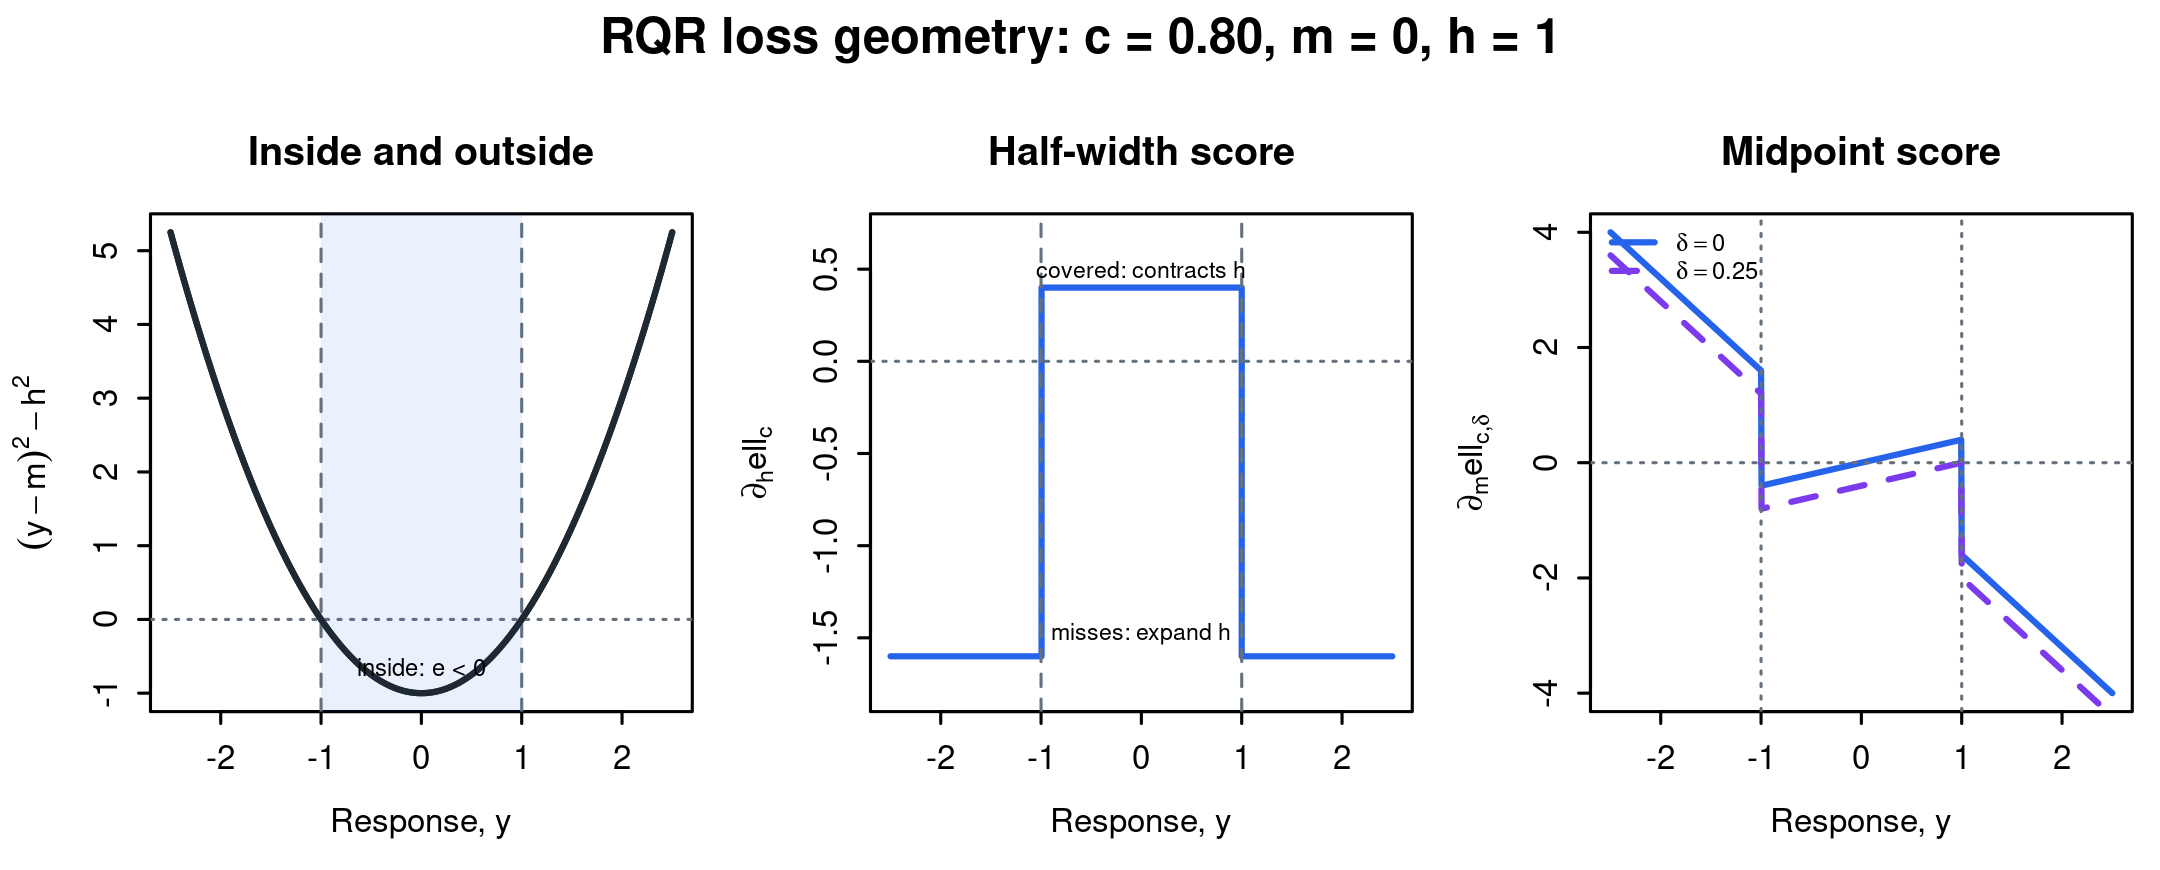
\includegraphics[width=\textwidth]{figures/generated/figS02_loss_geometry.png}
\caption{\textbf{MPI loss geometry and the fixed midpoint tilt.}
For \(c=0.80\), \(m=0\), and \(h=1\), the residual product is negative exactly
inside the interval. The half-width score contracts \(h\) for covered
observations and expands it for misses. A fixed \(\delta\) adds a constant
shift to the midpoint score but leaves the half-width score unchanged. These
plots use the strict convention \(\ind(e<0)\): filled endpoint marks show the
score at \(y=\pm1\), while open marks show the one-sided inside limits. These
are deterministic pointwise score calculations, not fitted results.}
\label{fig:supp-loss-geometry}
\end{figure}

\section{Width-Regularized Interval Loss}
\label{sec:supp-rqr-w}

The width-regularized variant in \citet{PouplinEtAl2024RQR} has a different
population score system from the MPI loss. For comparison, they use the RQR-W
population objective
\[
\E\left[\rho_q\{(Y-a)(Y-b)\}\right]
+\frac{\lambda_W}{2}(b-a)^2,
\qquad \lambda_W\ge0.
\]
In the present terminology, RQR-W is a width-regularized modification of the
MPI loss, not the MPI loss itself.
At a nondegenerate interior stationary point, subtracting the two endpoint
score equations gives
\[
\Pr(a<Y<b)=q-2\lambda_W.
\]
Thus \(q=c+2\lambda_W\) restores content \(c\), subject to
\(0\le\lambda_W<(1-c)/2\). The midpoint equation then gives
\[
\E(Y\mid a<Y<b)
=\mu+\frac{2\lambda_W}{c}(\mu-m),
\qquad m=\frac{a+b}{2}.
\]
Except in special symmetric cases, RQR-W therefore changes the
mean-preserving placement equation. It is a coverage-corrected compromise
between MPI risk and squared width, not a tie-breaker among
unidentified MPI minimizers.

More generally, if a differentiable width penalty \(P(w)\), \(w=b-a\), is
added to a check loss at level \(q\), the coverage equation is
\[
\Pr(a<Y<b)=q-\frac{2P'(w)}{w}.
\]
A correction independent of the distribution and realized width is possible
only when \(P'(w)/w\) is constant, which yields a quadratic penalty up to an
additive constant. This explains both the form of RQR-W and why its path does
not generally coincide with the shortest-contiguous path.


\section*{Part III. Fixed-Target Computation and Content Checking}

\section{Fixed-Target MTI-ECM Calculation}
\label{sec:supp-mti-ecm}

The MTI-ECM calculation used in the validation study is a deterministic mode
calculation for a fixed loss-defined target. It is included because it links the
tolerance comparison to the MTI generalized-Bayes construction. The calculation
updates an interval-root target under a loss; the distribution-free tolerance
certificate remains attached to TCSP.

For \(e_i=(y_i-\eta_{1i})(y_i-\eta_{2i})\), the fixed-target MTI loss is
\[
L_{n,q,\delta}
=\sum_{i=1}^n\left[
\rho_q(e_i)-q\delta(\eta_{1i}+\eta_{2i}-2y_i)
\right],
\qquad
\rho_q(r)=r\{q-\ind(r<0)\}.
\]
With fixed learning rate \(\omega_{\mathrm R}\), the generalized-posterior
kernel is proportional to
\[
\exp\{-\omega_{\mathrm R}L_{n,q,\delta}(\theta)\}\pi_0(\theta).
\]
The validation calculations are intercept-only, so \(\theta=(a,b)\) before the
two roots are sorted into lower and upper endpoints.

The pseudo-asymmetric-Laplace representation gives a convenient quadratic
conditional calculation. Define
\[
\sigma_{\mathrm R}=\omega_{\mathrm R}^{-1},\qquad
\xi_q=\frac{1-2q}{q(1-q)},\qquad
\phi_q=\frac{2}{q(1-q)}.
\]
Then
\begin{align}
&\frac{q(1-q)}{\sigma_{\mathrm R}}
\exp\{-\rho_q(e_i)/\sigma_{\mathrm R}\}\notag\\
&\quad=\int_0^\infty
\Normal\!\left(e_i\mid\xi_qv_i,\phi_q\sigma_{\mathrm R}v_i\right)
\Exp\!\left(v_i\mid\mathrm{rate}=1/\sigma_{\mathrm R}\right)\,dv_i.
\label{eq:supp-pseudo-al-mixture}
\end{align}
The latent scale is computational; it augments a loss factor rather than a
sampling distribution for \(Y_i\).

Under the \(\GIG(\nu,A,B)\) convention proportional to
\(v^{\nu-1}\exp\{-(Av+B/v)/2\}\), the conditional scale law has
\[
v_i\mid\cdot\sim
\GIG\left\{
\frac12,\
\frac{1}{2\sigma_{\mathrm R}q(1-q)},\
\frac{q(1-q)e_i^2}{2\sigma_{\mathrm R}}
\right\}.
\]
For \(e_i\ne0\),
\[
\tau_i=E(v_i^{-1}\mid\cdot)=\frac{1}{q(1-q)|e_i|}.
\]
The numerical ECM calculation uses a small response-product scale floor when
\(e_i\) is near zero, objective backtracking after each accepted cycle, and
deterministic multi-start selection by the exact penalized objective.

\begin{algorithmblock}{Fixed-target MTI-ECM mode}
\item Fix \(q\), \(\delta\), \(\omega_{\mathrm R}\), the ridge prior precision,
and deterministic starting roots.
\item At the current roots, compute product residuals \(e_i\) and inverse-scale
moments \(\tau_i\), using the prespecified numerical floor only when needed.
\item Holding one root fixed, solve the Gaussian conditional maximization for
the other root. Repeat with the roles exchanged.
\item Accept a full cycle only if the exact penalized objective decreases,
using backtracking if necessary.
\item Return the best deterministic mode over the prespecified starting values,
then sort the two raw roots to report the interval.
\end{algorithmblock}

The fitted content \(q\) and tilt \(\delta\) are not estimated as ordinary
parameters inside the generalized posterior. The validation study profiles over
a prespecified grid in a separate calibration step and then applies the selected
rule unchanged to independent replications.

\section{Direct DP Content Check}
\label{sec:supp-direct-dp-check}

The MTI-ECM comparator uses a model-based content-probability check during calibration.
For a fixed closed interval \(I=[l,u]\), let \(N_n(I)=\sum_{i=1}^n\ind(Y_i\in I)\).
Under the direct Dirichlet-process model
\[
F\sim\mathrm{DP}(a,H),\qquad
Y_i\mid F\stackrel{\mathrm{iid}}{\sim}F,
\]
with fixed \(a>0\) and fixed base distribution \(H\), conjugacy gives an exact
posterior law for the interval content.

\begin{proposition}[Direct DP fixed-interval content law]
\label{prop:supp-dp-content-law}
For fixed \(I=[l,u]\),
\[
F(I)\mid D_n\sim
\mathrm{Beta}\{aH(I)+N_n(I),a(1-H(I))+n-N_n(I)\}.
\]
Consequently \(p_n(I;c)=\Pr\{F(I)\ge c\mid D_n\}\) is available from a Beta
survival probability.
\end{proposition}

\begin{proof}
Dirichlet-process conjugacy gives
\[
F\mid D_n\sim \mathrm{DP}(a+n,H_n),\qquad
H_n=\frac{aH+\sum_{i=1}^n\delta_{Y_i}}{a+n}.
\]
For the partition \((I,I^c)\), the finite-dimensional distribution of a
Dirichlet process is Dirichlet with parameters
\((a+n)H_n(I)=aH(I)+N_n(I)\) and
\((a+n)H_n(I^c)=a\{1-H(I)\}+n-N_n(I)\). The first coordinate is the stated
Beta distribution.
\end{proof}

The direct DP check is used only to choose eligible MTI-ECM candidates in the
calibration run. Distribution-free tolerance certification in this paper comes
from the TCSP retained-count calibration.

\section*{Part IV. Validation Details and Reproducibility}

\section{Tolerance-Validation Protocol and Feasibility}
\label{sec:supp-tolerance-validation-protocol}

The primary tolerance validation is restricted to iid continuous univariate
samples. This is the setting in which the scan-calibrated empirical action,
the stability-restricted MTI-ECM profile rule, Young--Mathew interpolation, and
Wilks-style full-range intervals can be compared on the same target. TCSP
is the primary calibrated action
because it selects the shortest closed order-statistic window at the calibrated
retained count. The reported TCSP calculations use adaptive Clopper--Pearson scan
calibration directly. The MTI-ECM comparator
profiles fixed-target endpoint fits over fitted content and retained-mean tilt,
then applies a direct Dirichlet-process fixed-interval content probability
threshold and a width-stability restriction. Young--Mathew and Wilks are included as classical order-statistic
comparators. Regression and dynamic tolerance calibration require additional
results because the fitted intervals vary with covariates or time.

The simulation design fixes tolerance confidence \(1-\alpha=0.95\) and uses
explicit feasible design cells:
\[
  \begin{aligned}
  (n,c)\in\{&
  (50,0.90),(100,0.90),(100,0.95),\\
  &(500,0.90),(500,0.95),(500,0.99),\\
  &(1000,0.90),(1000,0.95),(1000,0.99)\}.
  \end{aligned}
\]
The distributional panel contains two symmetric reference distributions and six
asymmetric simulation distributions. The symmetric reference distributions are
Gaussian and Student \(t_3\). The asymmetric simulation distributions are
exponential, asymmetric Laplace with \(\tau=0.10\), two-piece Normal with scale
ratio \(1{:}12\), Beta\((1,8)\), Gamma\((0.5,1)\), and log-normal with
log-scale standard deviation \(1.25\). All laws are centered and scaled before
sampling. Each cell uses paired random samples across methods. The
reproducibility materials include the code version, simulation settings,
package versions, random seeds, calibration files, and numerical summaries.
The article comparison combines the completed TCSP, Young--Mathew, and Wilks
confirmatory run with the stability-restricted adaptive MTI-ECM profile rule applied to the
completed independent validation run. The reported rows contribute 288,000
replication-level method evaluations over the 72 distribution-level cells used in the main
comparison. The broader MTI-ECM refinement run is retained as calibration
evidence, with only the selected rule evaluated under the MTI-ECM label in the
independent validation run. All simulations completed, and all four reported methods returned
an interval in every replication. The manuscript tables and figures are
computed directly from these replication-level simulation outputs and the
corresponding scan-calibration outputs. The scenario-range table in the main
article is summarized across distributions within each \((n,c)\) cell, while
the supplement keeps the distribution-level content-attainment and width
summaries.
Table~\ref{tab:supp-primary-dgp-delivery} gives the distribution-level
content-attainment percentages before aggregation, and
Table~\ref{tab:supp-primary-dgp-width-ranges} reports the corresponding
distribution-level 2.5\%--97.5\% ranges of interval lengths. The
replication-level data file retains interval-return indicators,
infeasibility indicators, and raw width summaries for each
distribution-level cell as reproducibility information.

The MTI-ECM comparator reported in the main article uses a prespecified adaptive
calibration rule indexed by \((n,c,1-\alpha)\). The rule chooses a
direct Dirichlet-process content-probability check from a separate calibration run,
requires width stability relative to TCSP within the same distribution-level
cells, and then applies that choice unchanged to fresh paired replications in
the independent validation
run. Table~\ref{tab:supp-mti-ecm-policy} records the selected content-probability check, calibration
lower bound, independent validation range, and width span for each cell.

\begingroup
\TableStyle
\begin{longtable}{@{}>{\raggedright\arraybackslash}p{0.22\textwidth}rrrrrr@{}}
\caption{\textbf{Distribution-level tolerance-validation content attainment.} Entries are percentages of replications in which the produced interval attained the requested population content for the reported methods at tolerance confidence \(0.95\). Intervals not produced are counted as nonattainment.}\label{tab:supp-primary-dgp-delivery}\\
\toprule
Distribution & \(n\) & \(c\) & TCSP & MTI-ECM & Young--Mathew & Wilks
\\
\midrule
\endfirsthead
\toprule
Distribution & \(n\) & \(c\) & TCSP & MTI-ECM & Young--Mathew & Wilks
\\
\midrule
\endhead
Gaussian & 50 & 0.90 & 97.1 & 96.9 & 96.0 & 97.1
\\
Student t(3) & 50 & 0.90 & 97.1 & 96.9 & 96.7 & 97.1
\\
Exponential & 50 & 0.90 & 96.7 & 96.7 & 96.4 & 96.7
\\
Asymmetric Laplace (tau=0.10) & 50 & 0.90 & 95.9 & 96.1 & 95.5 & 95.9
\\
Two-piece Normal (1:12) & 50 & 0.90 & 96.6 & 97.4 & 95.9 & 96.6
\\
Beta(1,8) & 50 & 0.90 & 97.7 & 97.7 & 97.0 & 97.7
\\
Gamma(0.5,1) & 50 & 0.90 & 95.6 & 96.8 & 94.6 & 95.6
\\
Log-normal (log sd 1.25) & 50 & 0.90 & 96.4 & 95.7 & 96.1 & 96.4
\\
Gaussian & 100 & 0.90 & 99.1 & 89.0 & 96.9 & 100.0
\\
Student t(3) & 100 & 0.90 & 98.3 & 94.8 & 96.3 & 100.0
\\
Exponential & 100 & 0.90 & 99.2 & 97.8 & 95.2 & 100.0
\\
Asymmetric Laplace (tau=0.10) & 100 & 0.90 & 99.1 & 96.5 & 95.9 & 100.0
\\
Two-piece Normal (1:12) & 100 & 0.90 & 98.7 & 96.4 & 96.0 & 99.9
\\
Beta(1,8) & 100 & 0.90 & 98.9 & 97.3 & 96.1 & 99.9
\\
Gamma(0.5,1) & 100 & 0.90 & 99.4 & 98.4 & 96.8 & 100.0
\\
Log-normal (log sd 1.25) & 100 & 0.90 & 99.3 & 98.1 & 96.4 & 100.0
\\
Gaussian & 100 & 0.95 & 96.2 & 97.3 & 95.5 & 96.2
\\
Student t(3) & 100 & 0.95 & 96.8 & 95.6 & 96.0 & 96.8
\\
Exponential & 100 & 0.95 & 97.1 & 97.1 & 96.7 & 97.1
\\
Asymmetric Laplace (tau=0.10) & 100 & 0.95 & 97.2 & 96.0 & 96.6 & 97.2
\\
Two-piece Normal (1:12) & 100 & 0.95 & 97.3 & 95.4 & 96.7 & 97.3
\\
Beta(1,8) & 100 & 0.95 & 97.3 & 94.4 & 96.8 & 97.3
\\
Gamma(0.5,1) & 100 & 0.95 & 96.8 & 96.5 & 96.5 & 96.8
\\
Log-normal (log sd 1.25) & 100 & 0.95 & 96.7 & 96.4 & 96.3 & 96.7
\\
Gaussian & 500 & 0.90 & 96.7 & 95.5 & 95.6 & 100.0
\\
Student t(3) & 500 & 0.90 & 98.3 & 95.6 & 95.8 & 100.0
\\
Exponential & 500 & 0.90 & 99.0 & 98.5 & 94.5 & 100.0
\\
Asymmetric Laplace (tau=0.10) & 500 & 0.90 & 99.0 & 97.5 & 96.1 & 100.0
\\
Two-piece Normal (1:12) & 500 & 0.90 & 98.6 & 96.5 & 95.1 & 100.0
\\
Beta(1,8) & 500 & 0.90 & 99.0 & 98.6 & 94.4 & 100.0
\\
Gamma(0.5,1) & 500 & 0.90 & 98.8 & 98.9 & 94.8 & 100.0
\\
Log-normal (log sd 1.25) & 500 & 0.90 & 99.0 & 98.6 & 95.1 & 100.0
\\
Gaussian & 500 & 0.95 & 96.2 & 95.2 & 96.0 & 100.0
\\
Student t(3) & 500 & 0.95 & 97.4 & 96.5 & 96.6 & 100.0
\\
Exponential & 500 & 0.95 & 99.0 & 98.0 & 96.2 & 100.0
\\
Asymmetric Laplace (tau=0.10) & 500 & 0.95 & 98.0 & 96.5 & 95.1 & 100.0
\\
Two-piece Normal (1:12) & 500 & 0.95 & 97.2 & 96.7 & 94.4 & 100.0
\\
Beta(1,8) & 500 & 0.95 & 99.1 & 97.6 & 96.1 & 100.0
\\
Gamma(0.5,1) & 500 & 0.95 & 99.0 & 98.7 & 95.7 & 100.0
\\
Log-normal (log sd 1.25) & 500 & 0.95 & 98.9 & 98.5 & 94.2 & 100.0
\\
Gaussian & 500 & 0.99 & 96.4 & 96.1 & 95.8 & 96.4
\\
Student t(3) & 500 & 0.99 & 96.7 & 90.7 & 96.7 & 96.7
\\
Exponential & 500 & 0.99 & 96.6 & 95.7 & 96.3 & 96.6
\\
Asymmetric Laplace (tau=0.10) & 500 & 0.99 & 96.1 & 95.4 & 95.6 & 96.1
\\
Two-piece Normal (1:12) & 500 & 0.99 & 96.2 & 96.3 & 95.9 & 96.2
\\
Beta(1,8) & 500 & 0.99 & 95.5 & 94.7 & 95.1 & 95.5
\\
Gamma(0.5,1) & 500 & 0.99 & 95.3 & 96.7 & 95.1 & 95.3
\\
Log-normal (log sd 1.25) & 500 & 0.99 & 96.3 & 94.1 & 95.9 & 96.3
\\
Gaussian & 1000 & 0.90 & 98.0 & 95.1 & 95.3 & 100.0
\\
Student t(3) & 1000 & 0.90 & 98.6 & 94.8 & 94.2 & 100.0
\\
Exponential & 1000 & 0.90 & 99.6 & 98.3 & 96.1 & 100.0
\\
Asymmetric Laplace (tau=0.10) & 1000 & 0.90 & 98.6 & 95.2 & 95.2 & 100.0
\\
Two-piece Normal (1:12) & 1000 & 0.90 & 98.7 & 95.1 & 95.4 & 100.0
\\
Beta(1,8) & 1000 & 0.90 & 99.2 & 97.2 & 94.5 & 100.0
\\
Gamma(0.5,1) & 1000 & 0.90 & 99.5 & 97.7 & 96.1 & 100.0
\\
Log-normal (log sd 1.25) & 1000 & 0.90 & 99.6 & 97.4 & 96.6 & 100.0
\\
Gaussian & 1000 & 0.95 & 98.1 & 95.5 & 95.6 & 100.0
\\
Student t(3) & 1000 & 0.95 & 97.6 & 97.9 & 95.4 & 100.0
\\
Exponential & 1000 & 0.95 & 99.6 & 98.5 & 95.5 & 100.0
\\
Asymmetric Laplace (tau=0.10) & 1000 & 0.95 & 98.5 & 97.4 & 96.3 & 100.0
\\
Two-piece Normal (1:12) & 1000 & 0.95 & 98.8 & 98.0 & 95.1 & 100.0
\\
Beta(1,8) & 1000 & 0.95 & 99.3 & 98.5 & 95.1 & 100.0
\\
Gamma(0.5,1) & 1000 & 0.95 & 99.5 & 98.4 & 95.1 & 100.0
\\
Log-normal (log sd 1.25) & 1000 & 0.95 & 99.6 & 98.2 & 95.5 & 100.0
\\
Gaussian & 1000 & 0.99 & 97.5 & 93.1 & 96.9 & 99.9
\\
Student t(3) & 1000 & 0.99 & 98.8 & 95.0 & 96.9 & 100.0
\\
Exponential & 1000 & 0.99 & 99.5 & 97.2 & 97.2 & 100.0
\\
Asymmetric Laplace (tau=0.10) & 1000 & 0.99 & 99.0 & 95.7 & 96.8 & 100.0
\\
Two-piece Normal (1:12) & 1000 & 0.99 & 98.2 & 95.9 & 95.1 & 100.0
\\
Beta(1,8) & 1000 & 0.99 & 98.8 & 97.8 & 95.3 & 99.9
\\
Gamma(0.5,1) & 1000 & 0.99 & 98.9 & 98.1 & 96.4 & 99.9
\\
Log-normal (log sd 1.25) & 1000 & 0.99 & 99.2 & 96.5 & 94.1 & 100.0
\\
\bottomrule
\end{longtable}

\endgroup

\begingroup
\scriptsize
\begin{longtable}{@{}p{0.24\textwidth}rrp{0.20\textwidth}rr@{}}
\caption{\textbf{Primary iid tolerance-validation width ranges by DGP.} Width intervals are empirical 2.5\%--97.5\% ranges over the paired resamplings within each DGP, sample size, content, and method. Widths are not pooled across DGPs.}\label{tab:supp-primary-dgp-width-ranges}\\
\toprule
DGP & \(n\) & \(c\) & Method & Delivery (\%) & Width 95\% range\\
\midrule
\endfirsthead
\toprule
DGP & \(n\) & \(c\) & Method & Delivery (\%) & Width 95\% range\\
\midrule
\endhead
Beta(5,2) & 50 & 0.90 & TCSP & 95.7 & 3.16--5.06 \\
Beta(5,2) & 50 & 0.90 & Young--Mathew & 95.2 & 3.12--4.86 \\
Beta(5,2) & 50 & 0.90 & Wilks & 95.7 & 3.16--5.06 \\
contaminated normal & 50 & 0.90 & TCSP & 97.3 & 1.98--13.98 \\
contaminated normal & 50 & 0.90 & Young--Mathew & 96.9 & 1.93--12.68 \\
contaminated normal & 50 & 0.90 & Wilks & 97.3 & 1.98--13.98 \\
exponential & 50 & 0.90 & TCSP & 96.7 & 2.67--7.9 \\
exponential & 50 & 0.90 & Young--Mathew & 96.4 & 2.62--7.15 \\
exponential & 50 & 0.90 & Wilks & 96.7 & 2.67--7.9 \\
Gamma(2,1) & 50 & 0.90 & TCSP & 97.7 & 2.95--7.1 \\
Gamma(2,1) & 50 & 0.90 & Young--Mathew & 96.8 & 2.89--6.61 \\
Gamma(2,1) & 50 & 0.90 & Wilks & 97.7 & 2.95--7.1 \\
Gaussian & 50 & 0.90 & TCSP & 97.1 & 3.4--5.97 \\
Gaussian & 50 & 0.90 & Young--Mathew & 96.0 & 3.33--5.7 \\
Gaussian & 50 & 0.90 & Wilks & 97.1 & 3.4--5.97 \\
hard log-normal & 50 & 0.90 & TCSP & 96.4 & 1.41--14.4 \\
hard log-normal & 50 & 0.90 & Young--Mathew & 96.1 & 1.34--12.42 \\
hard log-normal & 50 & 0.90 & Wilks & 96.4 & 1.41--14.4 \\
Laplace & 50 & 0.90 & TCSP & 96.3 & 3.32--8.3 \\
Laplace & 50 & 0.90 & Young--Mathew & 95.7 & 3.26--7.73 \\
Laplace & 50 & 0.90 & Wilks & 96.3 & 3.32--8.3 \\
Student t3 & 50 & 0.90 & TCSP & 97.1 & 2.89--13.27 \\
Student t3 & 50 & 0.90 & Young--Mathew & 96.7 & 2.81--11.64 \\
Student t3 & 50 & 0.90 & Wilks & 97.1 & 2.89--13.27 \\
Beta(5,2) & 100 & 0.90 & TCSP & 98.8 & 3.25--4.47 \\
Beta(5,2) & 100 & 0.90 & Young--Mathew & 97.6 & 3.28--4.58 \\
Beta(5,2) & 100 & 0.90 & Wilks & 100.0 & 3.65--5.24 \\
contaminated normal & 100 & 0.90 & TCSP & 98.6 & 2--8.74 \\
contaminated normal & 100 & 0.90 & Young--Mathew & 96.8 & 1.95--8.45 \\
contaminated normal & 100 & 0.90 & Wilks & 100.0 & 2.86--16.84 \\
exponential & 100 & 0.90 & TCSP & 99.2 & 2.58--5.1 \\
exponential & 100 & 0.90 & Young--Mathew & 95.2 & 2.86--5.85 \\
exponential & 100 & 0.90 & Wilks & 100.0 & 3.3--8.24 \\
Gamma(2,1) & 100 & 0.90 & TCSP & 99.2 & 2.99--4.86 \\
Gamma(2,1) & 100 & 0.90 & Young--Mathew & 96.7 & 3.1--5.75 \\
Gamma(2,1) & 100 & 0.90 & Wilks & 100.0 & 3.53--7.37 \\
Gaussian & 100 & 0.90 & TCSP & 99.1 & 3.44--4.98 \\
Gaussian & 100 & 0.90 & Young--Mathew & 96.9 & 3.37--4.87 \\
Gaussian & 100 & 0.90 & Wilks & 100.0 & 3.95--6.24 \\
hard log-normal & 100 & 0.90 & TCSP & 99.3 & 1.43--5.47 \\
hard log-normal & 100 & 0.90 & Young--Mathew & 96.4 & 1.71--7.92 \\
hard log-normal & 100 & 0.90 & Wilks & 100.0 & 2.21--18.36 \\
Laplace & 100 & 0.90 & TCSP & 98.7 & 3.56--6.28 \\
Laplace & 100 & 0.90 & Young--Mathew & 98.5 & 3.48--6.15 \\
Laplace & 100 & 0.90 & Wilks & 100.0 & 4.36--9.49 \\
Student t3 & 100 & 0.90 & TCSP & 98.3 & 2.91--6.5 \\
Student t3 & 100 & 0.90 & Young--Mathew & 96.3 & 2.92--6.53 \\
Student t3 & 100 & 0.90 & Wilks & 100.0 & 3.86--17.44 \\
Beta(5,2) & 100 & 0.95 & TCSP & 95.5 & 3.63--5.25 \\
Beta(5,2) & 100 & 0.95 & Young--Mathew & 94.9 & 3.6--5.1 \\
Beta(5,2) & 100 & 0.95 & Wilks & 95.5 & 3.63--5.25 \\
contaminated normal & 100 & 0.95 & TCSP & 95.4 & 2.72--16.53 \\
contaminated normal & 100 & 0.95 & Young--Mathew & 95.3 & 2.67--15.45 \\
contaminated normal & 100 & 0.95 & Wilks & 95.4 & 2.72--16.53 \\
exponential & 100 & 0.95 & TCSP & 97.1 & 3.25--8.44 \\
exponential & 100 & 0.95 & Young--Mathew & 96.7 & 3.2--7.95 \\
exponential & 100 & 0.95 & Wilks & 97.1 & 3.25--8.44 \\
Gamma(2,1) & 100 & 0.95 & TCSP & 95.8 & 3.44--7.5 \\
Gamma(2,1) & 100 & 0.95 & Young--Mathew & 95.0 & 3.42--7.12 \\
Gamma(2,1) & 100 & 0.95 & Wilks & 95.8 & 3.44--7.5 \\
Gaussian & 100 & 0.95 & TCSP & 96.2 & 3.97--6.42 \\
Gaussian & 100 & 0.95 & Young--Mathew & 95.5 & 3.91--6.18 \\
Gaussian & 100 & 0.95 & Wilks & 96.2 & 3.97--6.42 \\
hard log-normal & 100 & 0.95 & TCSP & 96.7 & 2.3--16.67 \\
hard log-normal & 100 & 0.95 & Young--Mathew & 96.3 & 2.24--15.35 \\
hard log-normal & 100 & 0.95 & Wilks & 96.7 & 2.3--16.67 \\
Laplace & 100 & 0.95 & TCSP & 96.3 & 4.29--9.33 \\
Laplace & 100 & 0.95 & Young--Mathew & 95.7 & 4.26--8.9 \\
Laplace & 100 & 0.95 & Wilks & 96.3 & 4.29--9.33 \\
Student t3 & 100 & 0.95 & TCSP & 96.8 & 3.8--16.99 \\
Student t3 & 100 & 0.95 & Young--Mathew & 96.0 & 3.73--15.28 \\
Student t3 & 100 & 0.95 & Wilks & 96.8 & 3.8--16.99 \\
Beta(5,2) & 500 & 0.90 & TCSP & 98.1 & 3.13--3.55 \\
Beta(5,2) & 500 & 0.90 & Young--Mathew & 95.5 & 3.21--3.7 \\
Beta(5,2) & 500 & 0.90 & Wilks & 100.0 & 4.49--5.58 \\
contaminated normal & 500 & 0.90 & TCSP & 97.4 & 1.85--2.42 \\
contaminated normal & 500 & 0.90 & Young--Mathew & 95.8 & 1.82--2.38 \\
contaminated normal & 500 & 0.90 & Wilks & 100.0 & 10.36--21.23 \\
exponential & 500 & 0.90 & TCSP & 99.0 & 2.4--3.05 \\
exponential & 500 & 0.90 & Young--Mathew & 94.5 & 2.83--3.71 \\
exponential & 500 & 0.90 & Wilks & 100.0 & 4.87--10.39 \\
Gamma(2,1) & 500 & 0.90 & TCSP & 98.5 & 2.76--3.32 \\
Gamma(2,1) & 500 & 0.90 & Young--Mathew & 96.0 & 3.04--3.79 \\
Gamma(2,1) & 500 & 0.90 & Wilks & 100.0 & 4.88--8.88 \\
Gaussian & 500 & 0.90 & TCSP & 96.7 & 3.31--3.86 \\
Gaussian & 500 & 0.90 & Young--Mathew & 95.6 & 3.26--3.84 \\
Gaussian & 500 & 0.90 & Wilks & 100.0 & 5.17--7.28 \\
hard log-normal & 500 & 0.90 & TCSP & 99.0 & 1.24--1.9 \\
hard log-normal & 500 & 0.90 & Young--Mathew & 95.1 & 1.68--2.8 \\
hard log-normal & 500 & 0.90 & Wilks & 100.0 & 5.03--29.37 \\
Laplace & 500 & 0.90 & TCSP & 97.5 & 3.29--4.14 \\
Laplace & 500 & 0.90 & Young--Mathew & 95.8 & 3.21--4.08 \\
Laplace & 500 & 0.90 & Wilks & 100.0 & 6.64--11.23 \\
Student t3 & 500 & 0.90 & TCSP & 98.3 & 2.77--3.62 \\
Student t3 & 500 & 0.90 & Young--Mathew & 95.8 & 2.69--3.54 \\
Student t3 & 500 & 0.90 & Wilks & 100.0 & 6.91--25.85 \\
Beta(5,2) & 500 & 0.95 & TCSP & 97.7 & 3.63--4.15 \\
Beta(5,2) & 500 & 0.95 & Young--Mathew & 95.9 & 3.71--4.36 \\
Beta(5,2) & 500 & 0.95 & Wilks & 100.0 & 4.46--5.61 \\
contaminated normal & 500 & 0.95 & TCSP & 98.3 & 2.6--6.88 \\
contaminated normal & 500 & 0.95 & Young--Mathew & 96.9 & 2.53--6.77 \\
contaminated normal & 500 & 0.95 & Wilks & 100.0 & 10.16--21.21 \\
exponential & 500 & 0.95 & TCSP & 99.0 & 3.11--4.17 \\
exponential & 500 & 0.95 & Young--Mathew & 96.2 & 3.56--4.92 \\
exponential & 500 & 0.95 & Wilks & 100.0 & 4.96--9.51 \\
Gamma(2,1) & 500 & 0.95 & TCSP & 98.2 & 3.4--4.31 \\
Gamma(2,1) & 500 & 0.95 & Young--Mathew & 96.0 & 3.69--4.84 \\
Gamma(2,1) & 500 & 0.95 & Wilks & 100.0 & 4.89--9 \\
Gaussian & 500 & 0.95 & TCSP & 96.2 & 3.91--4.67 \\
Gaussian & 500 & 0.95 & Young--Mathew & 96.0 & 3.9--4.66 \\
Gaussian & 500 & 0.95 & Wilks & 100.0 & 5.19--7.3 \\
hard log-normal & 500 & 0.95 & TCSP & 98.9 & 1.95--3.55 \\
hard log-normal & 500 & 0.95 & Young--Mathew & 94.2 & 2.49--5.18 \\
hard log-normal & 500 & 0.95 & Wilks & 100.0 & 4.91--30.5 \\
Laplace & 500 & 0.95 & TCSP & 98.2 & 4.33--5.65 \\
Laplace & 500 & 0.95 & Young--Mathew & 97.2 & 4.25--5.61 \\
Laplace & 500 & 0.95 & Wilks & 100.0 & 6.49--11.54 \\
Student t3 & 500 & 0.95 & TCSP & 97.4 & 3.73--5.38 \\
Student t3 & 500 & 0.95 & Young--Mathew & 96.6 & 3.7--5.34 \\
Student t3 & 500 & 0.95 & Wilks & 100.0 & 6.9--26.52 \\
Beta(5,2) & 500 & 0.99 & TCSP & 95.3 & 4.46--5.59 \\
Beta(5,2) & 500 & 0.99 & Young--Mathew & 94.6 & 4.44--5.52 \\
Beta(5,2) & 500 & 0.99 & Wilks & 95.3 & 4.46--5.59 \\
contaminated normal & 500 & 0.99 & TCSP & 95.7 & 9.97--21.36 \\
contaminated normal & 500 & 0.99 & Young--Mathew & 95.2 & 9.9--20.72 \\
contaminated normal & 500 & 0.99 & Wilks & 95.7 & 9.97--21.36 \\
exponential & 500 & 0.99 & TCSP & 96.6 & 4.96--9.98 \\
exponential & 500 & 0.99 & Young--Mathew & 96.3 & 4.92--9.61 \\
exponential & 500 & 0.99 & Wilks & 96.6 & 4.96--9.98 \\
Gamma(2,1) & 500 & 0.99 & TCSP & 95.3 & 4.9--8.89 \\
Gamma(2,1) & 500 & 0.99 & Young--Mathew & 95.0 & 4.88--8.56 \\
Gamma(2,1) & 500 & 0.99 & Wilks & 95.3 & 4.9--8.89 \\
Gaussian & 500 & 0.99 & TCSP & 96.4 & 5.18--7.28 \\
Gaussian & 500 & 0.99 & Young--Mathew & 95.8 & 5.17--7.17 \\
Gaussian & 500 & 0.99 & Wilks & 96.4 & 5.18--7.28 \\
hard log-normal & 500 & 0.99 & TCSP & 96.3 & 4.93--32.87 \\
hard log-normal & 500 & 0.99 & Young--Mathew & 95.9 & 4.84--31.39 \\
hard log-normal & 500 & 0.99 & Wilks & 96.3 & 4.93--32.87 \\
Laplace & 500 & 0.99 & TCSP & 95.1 & 6.58--11.67 \\
Laplace & 500 & 0.99 & Young--Mathew & 94.6 & 6.54--11.28 \\
Laplace & 500 & 0.99 & Wilks & 95.1 & 6.58--11.67 \\
Student t3 & 500 & 0.99 & TCSP & 96.7 & 7.01--26.46 \\
Student t3 & 500 & 0.99 & Young--Mathew & 96.7 & 6.93--25.28 \\
Student t3 & 500 & 0.99 & Wilks & 96.7 & 7.01--26.46 \\
Beta(5,2) & 1000 & 0.90 & TCSP & 97.8 & 3.11--3.42 \\
Beta(5,2) & 1000 & 0.90 & Young--Mathew & 95.7 & 3.21--3.56 \\
Beta(5,2) & 1000 & 0.90 & Wilks & 100.0 & 4.7--5.71 \\
contaminated normal & 1000 & 0.90 & TCSP & 98.9 & 1.86--2.2 \\
contaminated normal & 1000 & 0.90 & Young--Mathew & 95.8 & 1.82--2.15 \\
contaminated normal & 1000 & 0.90 & Wilks & 100.0 & 13.11--23.07 \\
exponential & 1000 & 0.90 & TCSP & 99.6 & 2.37--2.8 \\
exponential & 1000 & 0.90 & Young--Mathew & 96.1 & 2.85--3.44 \\
exponential & 1000 & 0.90 & Wilks & 100.0 & 5.58--10.42 \\
Gamma(2,1) & 1000 & 0.90 & TCSP & 99.6 & 2.78--3.16 \\
Gamma(2,1) & 1000 & 0.90 & Young--Mathew & 96.2 & 3.04--3.54 \\
Gamma(2,1) & 1000 & 0.90 & Wilks & 100.0 & 5.5--9.2 \\
Gaussian & 1000 & 0.90 & TCSP & 98.0 & 3.32--3.69 \\
Gaussian & 1000 & 0.90 & Young--Mathew & 95.3 & 3.27--3.65 \\
Gaussian & 1000 & 0.90 & Wilks & 100.0 & 5.63--7.6 \\
hard log-normal & 1000 & 0.90 & TCSP & 99.6 & 1.23--1.62 \\
hard log-normal & 1000 & 0.90 & Young--Mathew & 96.6 & 1.71--2.4 \\
hard log-normal & 1000 & 0.90 & Wilks & 100.0 & 6.5--40.48 \\
Laplace & 1000 & 0.90 & TCSP & 98.0 & 3.3--3.88 \\
Laplace & 1000 & 0.90 & Young--Mathew & 95.7 & 3.22--3.82 \\
Laplace & 1000 & 0.90 & Wilks & 100.0 & 7.51--12.76 \\
Student t3 & 1000 & 0.90 & TCSP & 98.6 & 2.77--3.33 \\
Student t3 & 1000 & 0.90 & Young--Mathew & 94.2 & 2.69--3.24 \\
Student t3 & 1000 & 0.90 & Wilks & 100.0 & 8.88--34.51 \\
Beta(5,2) & 1000 & 0.95 & TCSP & 99.0 & 3.62--3.99 \\
Beta(5,2) & 1000 & 0.95 & Young--Mathew & 97.2 & 3.72--4.13 \\
Beta(5,2) & 1000 & 0.95 & Wilks & 100.0 & 4.74--5.68 \\
contaminated normal & 1000 & 0.95 & TCSP & 98.7 & 2.52--5.38 \\
contaminated normal & 1000 & 0.95 & Young--Mathew & 95.1 & 2.42--4.78 \\
contaminated normal & 1000 & 0.95 & Wilks & 100.0 & 12.95--22.94 \\
exponential & 1000 & 0.95 & TCSP & 99.6 & 3.11--3.77 \\
exponential & 1000 & 0.95 & Young--Mathew & 95.5 & 3.56--4.42 \\
exponential & 1000 & 0.95 & Wilks & 100.0 & 5.6--10.99 \\
Gamma(2,1) & 1000 & 0.95 & TCSP & 99.0 & 3.42--3.98 \\
Gamma(2,1) & 1000 & 0.95 & Young--Mathew & 95.2 & 3.69--4.42 \\
Gamma(2,1) & 1000 & 0.95 & Wilks & 100.0 & 5.48--9.48 \\
Gaussian & 1000 & 0.95 & TCSP & 98.1 & 3.95--4.45 \\
Gaussian & 1000 & 0.95 & Young--Mathew & 95.6 & 3.9--4.4 \\
Gaussian & 1000 & 0.95 & Wilks & 100.0 & 5.6--7.68 \\
hard log-normal & 1000 & 0.95 & TCSP & 99.6 & 1.97--2.9 \\
hard log-normal & 1000 & 0.95 & Young--Mathew & 95.5 & 2.56--4.03 \\
hard log-normal & 1000 & 0.95 & Wilks & 100.0 & 6.84--40.05 \\
Laplace & 1000 & 0.95 & TCSP & 97.9 & 4.3--5.17 \\
Laplace & 1000 & 0.95 & Young--Mathew & 94.8 & 4.21--5.08 \\
Laplace & 1000 & 0.95 & Wilks & 100.0 & 7.54--12.8 \\
Student t3 & 1000 & 0.95 & TCSP & 97.6 & 3.71--4.84 \\
Student t3 & 1000 & 0.95 & Young--Mathew & 95.4 & 3.63--4.69 \\
Student t3 & 1000 & 0.95 & Wilks & 100.0 & 8.66--37.39 \\
Beta(5,2) & 1000 & 0.99 & TCSP & 98.0 & 4.46--5.19 \\
Beta(5,2) & 1000 & 0.99 & Young--Mathew & 96.6 & 4.54--5.33 \\
Beta(5,2) & 1000 & 0.99 & Wilks & 100.0 & 4.73--5.69 \\
contaminated normal & 1000 & 0.99 & TCSP & 98.1 & 10.7--17.56 \\
contaminated normal & 1000 & 0.99 & Young--Mathew & 97.3 & 10.56--17.32 \\
contaminated normal & 1000 & 0.99 & Wilks & 100.0 & 13.03--23.77 \\
exponential & 1000 & 0.99 & TCSP & 99.5 & 4.98--7.28 \\
exponential & 1000 & 0.99 & Young--Mathew & 97.2 & 5.28--8.18 \\
exponential & 1000 & 0.99 & Wilks & 100.0 & 5.6--10.39 \\
Gamma(2,1) & 1000 & 0.99 & TCSP & 99.0 & 4.94--6.92 \\
Gamma(2,1) & 1000 & 0.99 & Young--Mathew & 95.8 & 5.11--7.44 \\
Gamma(2,1) & 1000 & 0.99 & Wilks & 100.0 & 5.48--9.12 \\
Gaussian & 1000 & 0.99 & TCSP & 97.5 & 5.21--6.41 \\
Gaussian & 1000 & 0.99 & Young--Mathew & 96.9 & 5.19--6.42 \\
Gaussian & 1000 & 0.99 & Wilks & 99.9 & 5.61--7.65 \\
hard log-normal & 1000 & 0.99 & TCSP & 99.2 & 5.1--13.21 \\
hard log-normal & 1000 & 0.99 & Young--Mathew & 94.1 & 5.52--17.47 \\
hard log-normal & 1000 & 0.99 & Wilks & 100.0 & 6.37--39.88 \\
Laplace & 1000 & 0.99 & TCSP & 98.3 & 6.71--9.41 \\
Laplace & 1000 & 0.99 & Young--Mathew & 97.1 & 6.66--9.38 \\
Laplace & 1000 & 0.99 & Wilks & 99.9 & 7.65--12.11 \\
Student t3 & 1000 & 0.99 & TCSP & 98.8 & 7.26--14.48 \\
Student t3 & 1000 & 0.99 & Young--Mathew & 96.9 & 7.17--14.7 \\
Student t3 & 1000 & 0.99 & Wilks & 100.0 & 8.8--34.22 \\
\bottomrule
\end{longtable}
\endgroup


These results are empirical repeated-sampling evidence for the selected
profile rule; the finite-sample distribution-free certificate remains attached
to TCSP.

\begingroup
\scriptsize
\setlength{\tabcolsep}{3pt}
\begin{longtable}{@{}>{\raggedright\arraybackslash}p{0.16\textwidth}>{\centering\arraybackslash}p{0.12\textwidth}>{\centering\arraybackslash}p{0.17\textwidth}>{\centering\arraybackslash}p{0.16\textwidth}>{\centering\arraybackslash}p{0.12\textwidth}>{\centering\arraybackslash}p{0.19\textwidth}@{}}
\caption{\textbf{Selected adaptive MTI-ECM calibration rule.} The direct-DP content screen is fixed by a separate calibration run within each sample-size/content cell before the independent validation summaries are computed. Validation attainment is reported as the range across the eight simulation distributions.}\label{tab:supp-mti-ecm-policy}\\
\toprule
Cell & DP screen & Calibration lower probability & Validation range (\%) & Cells below 95\% & Width 95\% span
\\
\midrule
\endfirsthead
\toprule
Cell & DP screen & Calibration lower probability & Validation range (\%) & Cells below 95\% & Width 95\% span
\\
\midrule
\endhead
\(n=50,c=0.90\) & 0.995 & 0.966 & 96.3--97.7 & 0 & 1.48--15.12 \\
\(n=100,c=0.90\) & 0.995 & 0.986 & 98.1--99.3 & 0 & 1.48--5.49 \\
\(n=100,c=0.95\) & 0.995 & 0.962 & 95.8--97.8 & 0 & 2.29--18.69 \\
\(n=500,c=0.90\) & 0.995 & 0.983 & 97.1--99.7 & 0 & 1.26--3.86 \\
\(n=500,c=0.95\) & 0.995 & 0.983 & 97.6--99.3 & 0 & 2.03--5.43 \\
\(n=500,c=0.99\) & 0.995 & 0.954 & 95.1--96.5 & 0 & 4.57--30.7 \\
\(n=1000,c=0.90\) & 0.995 & 0.985 & 97.8--99.6 & 0 & 1.22--3.68 \\
\(n=1000,c=0.95\) & 0.995 & 0.987 & 97.5--99.5 & 0 & 1.97--4.74 \\
\(n=1000,c=0.99\) & 0.996 & 0.984 & 97.9--99.2 & 0 & 4.56--13.83 \\
\bottomrule
\end{longtable}
\endgroup


The TCSP calibration chooses the retained count \(k\) before seeing the
replicated samples. Table~\ref{tab:supp-tcsp-scan-calibration} records the
retained counts, retained fractions, content buffers, and certified lower
probabilities used in the simulation design. Adaptive Clopper--Pearson calibration
certifies the retained count for each feasible sample-size/content cell before
any distribution-specific replications are evaluated. When \(k=n\), TCSP is forced to
use the full sample range and therefore coincides with Wilks at the
formal-action level. This occurs for \((n,c)=(50,0.90),(100,0.95)\), and
\((500,0.99)\).

\begin{table}[H]
\centering
\caption{\textbf{TCSP scan calibration for the simulation design.} The retained
count \(k\) is selected by adaptive Clopper--Pearson Monte Carlo scan
calibration. The content buffer is \(k/n-c\).}
\label{tab:supp-tcsp-scan-calibration}
\TableStyle
\begin{tabular}{@{}rrrrrr@{}}
\toprule
\(n\) & \(c\) & Retained count \(k\) & \(k/n\) & Buffer \(k/n-c\) & Certified lower probability\\
\midrule
50 & 0.90 & 50 & 1.000 & 0.100 & 0.966 \\
100 & 0.90 & 98 & 0.980 & 0.080 & 0.964 \\
100 & 0.95 & 100 & 1.000 & 0.050 & 0.963 \\
500 & 0.90 & 468 & 0.936 & 0.036 & 0.951 \\
500 & 0.95 & 488 & 0.976 & 0.026 & 0.955 \\
500 & 0.99 & 500 & 1.000 & 0.010 & 0.960 \\
1000 & 0.90 & 926 & 0.926 & 0.026 & 0.955 \\
1000 & 0.95 & 969 & 0.969 & 0.019 & 0.960 \\
1000 & 0.99 & 998 & 0.998 & 0.008 & 0.960 \\
\bottomrule
\end{tabular}

\end{table}

Small-sample feasibility is governed by the full-range two-sided order-statistic
coverage probability
\[
  \Pr\{Y_{(1)}\le Y_{\mathrm{new}}\le Y_{(n)}
       \text{ for at least content } c\}
  =
  1-n(1-c)c^{n-1}-c^n .
\]
The smallest \(n\) satisfying this inequality depends on both content and
tolerance confidence. Table~\ref{tab:supp-full-range-thresholds} lists the
thresholds used to design the simulation study.

\begin{table}[H]
\centering
\caption{\textbf{Full-range feasibility thresholds.} Entries are the smallest
sample sizes for which the full-sample interval \([Y_{(1)},Y_{(n)}]\) reaches
the stated two-sided distribution-free content/confidence pair.}
\label{tab:supp-full-range-thresholds}
\TableStyle
\begin{tabular}{@{}lrrr@{}}
\toprule
Tolerance confidence & \(c=0.90\) & \(c=0.95\) & \(c=0.99\)\\
\midrule
\(0.90\) & 38 & 77 & 388\\
\(0.95\) & 46 & 93 & 473\\
\bottomrule
\end{tabular}
\end{table}

This distinction matters for interpreting the small sample sizes in
\citet{PourmohamadRichardsonSanso2026CalibratedBNP}. The values
\((38,77,388)\) are appropriate at \(90\%\) tolerance confidence. A
\(95\%\)-confidence design needs the larger thresholds \((46,93,473)\). The
simulation design therefore lists the feasible cells explicitly instead of
forming a Cartesian product of sample sizes and contents. This prevents the
comparison from treating structural infeasibility as a method failure.
The Young--Mathew comparator is evaluated through the \texttt{tolerance}
package's \texttt{nptol.int(..., method = "YM")} function. The completed
run used \texttt{tolerance} version 3.0.0, and the package version is included
in the method reproducibility record.


\section{Reproducibility and Validation Limits}
\label{sec:supp-reproducibility}

The reproducibility materials separate mathematical statements, numerical
construction, and repeated-sampling evidence. The proofs above support the
population MPI and MTI identities, the fractional empirical score balance, and
the direct DP fixed-interval content law under their stated assumptions. The
TCSP retained counts are calibrated before the replicated samples are analyzed.
The MTI-ECM content-probability check and stability rule are selected in a separate
calibration run and then applied unchanged in the independent validation run.

The validation evidence is confined to iid continuous univariate samples from
the prespecified simulation distributions. It does not establish tolerance
validity for regression intervals, dynamic endpoint states, dependent samples,
or response-predictive distributions. Those extensions require their own
targets, assumptions, algorithms, diagnostics, and validation designs.

\bibliographystyle{plainnat}
\bibliography{refs}

\end{document}
